\documentclass[11pt,a4paper]{article}

\usepackage[a4paper,margin=21mm]{geometry}
\usepackage{mathptmx}
\usepackage[T1]{fontenc}
\usepackage[utf8]{inputenc}
\usepackage{microtype}
\usepackage{graphicx}
\usepackage{booktabs}
\usepackage{tabularx}
\usepackage{amsmath,amssymb}
\usepackage{xcolor}
\usepackage[numbers,sort&compress]{natbib}
\usepackage{caption}
\usepackage{fancyhdr}
\usepackage{hyperref}

\definecolor{primary}{RGB}{24,78,119}
\definecolor{accent}{RGB}{184,29,52}
\definecolor{muted}{RGB}{90,98,106}

\hypersetup{
  colorlinks=true,
  linkcolor=primary,
  citecolor=primary,
  urlcolor=primary,
  pdftitle={Plasmid Localization and Last-Resort Antimicrobial Resistance Across Human, Livestock, and Wastewater Sectors: A Complete-Genome Study from 50 Countries},
  pdfauthor={Muhammad Ahmad Khan}
}

\setlength{\parskip}{5.2pt plus 1.5pt minus 1pt}
\setlength{\parindent}{0pt}

\captionsetup{
  font=small,
  labelfont={bf,color=primary},
  skip=6pt
}

\pagestyle{fancy}
\fancyhf{}
\fancyhead[L]{\footnotesize\color{muted}\textit{Plasmid Localization and Last-Resort AMR Across One Health Sectors}}
\fancyhead[R]{\footnotesize\color{muted}Khan (2026)}
\fancyfoot[C]{\footnotesize\thepage}
\renewcommand{\headrulewidth}{0.4pt}

\newcommand{\takeaway}[2]{%
  \vspace{6pt}\noindent\colorbox{primary!7}{%
    \parbox{\dimexpr\linewidth-2\fboxsep\relax}{%
      \vspace{3pt}\textbf{\color{primary}#1:}\hspace{0.4em}#2\vspace{3pt}%
    }%
  }\vspace{6pt}%
}

\begin{document}

% ==================== TITLE BLOCK ====================
\begin{center}
  {\LARGE\bfseries\color{primary} Plasmid Localization and Last-Resort Antimicrobial Resistance Across Human, Livestock, and Wastewater Sectors: A Complete-Genome Study from 50 Countries\par}
  \vspace{10pt}
  {\large Muhammad Ahmad Khan$^{1,*}$\par}
  \vspace{4pt}
  {\small\color{muted} $^{1}$Center of Biotechnology and Microbiology (COBAM), University of Peshawar, Khyber Pakhtunkhwa, Pakistan\\
  $^{*}$Correspondence: Center of Biotechnology and Microbiology, University of Peshawar, Pakistan\par}
\end{center}

\vspace{4pt}
\noindent\rule{\linewidth}{0.6pt}

% ==================== ABSTRACT ====================
\begin{abstract}
\noindent\textbf{Background:} Short-read assemblies dominate public antimicrobial resistance (AMR) repositories and often fragment plasmid-borne resistance loci, while unfiltered annotation outputs mix chromosomal virulence, stress, and intrinsic genes with acquired determinants.

\noindent\textbf{Methods:} We audited 433,603 \textit{Escherichia coli}/\textit{Shigella} and \textit{Klebsiella pneumoniae} assemblies from 151 countries in NCBI Pathogen Detection (2015--2026) across Human, Livestock/Poultry, and Wastewater/Aquatic sectors. Across 8,987 complete or chromosome-level assemblies from countries with multi-sector coverage, we fitted mixed-effects logistic models for last-resort resistance (carbapenemase or \textit{mcr}), including \textit{mcr}-only, income-stratified, and top-3-country-excluded sensitivity models. We then drew a fixed-seed stratified sample of one complete genome per country $\times$ species $\times$ sector stratum across 50 countries ($n = 150$ passing quality control) to quantify acquired-AMR plasmid localization and MOB-suite plasmid lineage overlap with permutation testing.

\noindent\textbf{Results:} Only 10,073 assemblies (2.3\%) were complete or chromosome-level, with lower low- and middle-income country (LMIC) counts in every sector (196 vs.\ 534 in wastewater). Across the 8,987-genome frame, last-resort carriage (6.57\%; 75.9\% \textit{mcr}) was consistently elevated in Livestock/Poultry overall (OR 3.04, 95\% CI 2.38--3.87), for \textit{mcr} alone (OR 3.43), in LMICs (OR 2.64), in HICs (OR 3.63), and after excluding the UK, China, and USA (OR 6.72). LMIC odds were higher overall (OR 3.31, 95\% CI 1.04--10.57) but attenuated with wider uncertainty when those three countries were removed (OR 2.63, 95\% CI 0.61--11.34). In the 150-genome sample, strictly acquired AMR genes were 78.6\% plasmid-borne (1,079/1,372), with \textit{bla}\textsubscript{NDM-5} (10/10) and \textit{bla}\textsubscript{KPC-2} (8/8) each carried across 5 independent plasmid clusters (cluster-level Wilson 95\% CI 0.57--1.00). Removing non-AMR and intrinsic hits reduced the \textit{K.~pneumoniae} vs.\ \textit{E.~coli} localization OR from 10.26 to 2.58 (95\% CI 1.10--6.04; deduplicated OR 2.76), with no detected sector or income difference. Non-singleton acquired-AMR plasmid clusters spanned sectors at rates matching random assortment (28/34 primary, $p = 0.757$; 26/33 secondary, $p = 0.452$).

\noindent\textbf{Conclusions:} Livestock reservoirs consistently show elevated last-resort AMR---driven predominantly by \textit{mcr}---across complete-genome frames, while acquired-AMR plasmid localization depends primarily on gene and species once non-AMR and intrinsic loci are excluded.
\end{abstract}

\noindent\textbf{Keywords:} One Health; Antimicrobial Resistance; Plasmid Localization Index; MOB-suite; \textit{Escherichia coli}; \textit{Klebsiella pneumoniae}; Complete Genomes.

\vspace{2pt}
\noindent\rule{\linewidth}{0.6pt}

% ==================== 1. INTRODUCTION ====================
\section{Introduction}

Bacterial antimicrobial resistance (AMR) was associated with 4.71 million deaths and directly attributable to 1.14 million deaths across 204 countries and territories in 2021, with low- and middle-income countries (LMICs) bearing the heaviest mortality \cite{naghavi2024}. Carbapenem-resistant and third-generation cephalosporin-resistant Enterobacterales---principally \textit{Escherichia coli} and \textit{Klebsiella pneumoniae}---sit in the Critical Priority tier of the 2024 World Health Organization Bacterial Priority Pathogens List \cite{who2024}.

Understanding how resistance moves across human, agricultural, and environmental interfaces requires measuring cross-sector connectivity rather than surveying compartments separately \cite{arnold2024,li2025}. Li et al.\ \cite{li2025} proposed four connectivity levels covering ecological overlap (L1), shared microbial lineages (L2), shared resistance gene repertoires (L3), and mobile genetic element (MGE) or plasmid sharing (L4). Empirical plasmid studies show that host strains and mobile elements often follow distinct trajectories: in the East of England, Ludden et al.\ \cite{ludden2019} found distinct \textit{E.~coli} populations and limited MGE overlap between human bloodstream infections and livestock, whereas global plasmidome mapping by Redondo-Salvo et al.\ \cite{redondosalvo2020} found that more than 60\% of mapped plasmids belong to plasmid taxonomic units (PTUs) with host ranges beyond a single species, and Acman et al.\ \cite{acman2022} reconstructed multi-layered plasmid and transposon mobilization driving global \textit{bla}\textsubscript{NDM} spread. Recent LMIC and high-income country (HIC) field studies---including ESBL-producing \textit{E.~coli} across humans, poultry, and wastewater in Douala, Cameroon \cite{djokonono2026} and national One Health genomic surveillance in Australia \cite{watt2025}---highlight both the value and practical hurdles of cross-sector genomic surveillance.

Two methodological problems still distort comparative plasmid analyses. First, short-read assemblies dominate public repositories; repetitive insertion sequences flanking carbapenemase (\textit{bla}\textsubscript{NDM}, \textit{bla}\textsubscript{KPC}, \textit{bla}\textsubscript{OXA-48}) and mobilized colistin resistance (\textit{mcr-1}) genes frequently break plasmid contigs into short fragments that plasmid classifiers assign to chromosomes. Second, automated annotation tools run with extended stress and virulence modules---such as AMRFinderPlus with \texttt{--plus} \cite{feldgarden2021}---report thousands of chromosomal virulence factors, metal/acid stress operons, chromosomal point mutations, and species-intrinsic chromosomal genes (\textit{bla}\textsubscript{EC}, \textit{emrD}, \textit{fosA}, \textit{oqxAB}, narrow-spectrum \textit{bla}\textsubscript{SHV}) alongside horizontally acquired resistance genes. Modeling plasmid localization on unfiltered outputs introduces strong taxonomic bias.

Here we audit 433,603 \textit{E.~coli}/\textit{Shigella} and \textit{K.~pneumoniae} assemblies across 151 countries, evaluate frame-level last-resort resistance models across 8,987 complete genomes, and analyze a fixed-seed stratified sample of 150 quality-controlled complete genomes from 50 countries to quantify acquired-AMR plasmid localization, clonal relatedness, and MOB-suite plasmid lineage overlap with per-plasmid cargo resolution and permutation testing.

% ==================== 2. METHODS ====================
\section{Methods}

\subsection{Repository Audit and Metadata Standardization}

Metadata and NCBI-generated AMRFinderPlus genotypes were downloaded from the \href{https://www.ncbi.nlm.nih.gov/pathogens/docs/isolates_gcp}{NCBI Pathogen Detection} FTP repository on 23 November 2026 for \textit{E.~coli}/\textit{Shigella} (\texttt{PDG000000004.6463}, 557.5~MB) and \textit{Klebsiella} (\texttt{PDG000000012.2587}, 196.8~MB, filtered to \texttt{scientific\_name = 'Klebsiella pneumoniae'}). Records from 2015--2026 with assembly accession, geographic location, and AMRFinderPlus version were retained ($n = 433{,}603$ distinct assemblies across 151 countries).

One Health sector assignment (\texttt{Human}, \texttt{Livestock\_Poultry}, \texttt{Wastewater\_Aquatic}) used a word-boundary-enforced regular expression classifier refined on an exploratory 50-genome Pakistan pilot (Supplementary Note). Bare \texttt{water} and unanchored \texttt{stream} tokens were removed so \texttt{midstream urine} did not map to aquatic sources; non-human hosts were evaluated before \texttt{epi\_type = 'clinical'}, and \texttt{Human} required explicit human host or clinical tissue attribution. Countries were mapped to World Bank income groups via the \href{https://api.worldbank.org/v2/country/all?format=json&per_page=300}{World Bank API} (24 November 2026), pooling LIC, LMC, and UMC economies as LMICs against HICs, with unmatched territories retained as \texttt{Unclassified}. Eligible assemblies were partitioned into the complete-genome audit (\texttt{Complete Genome} or \texttt{Chromosome}, $n = 10{,}073$) and a high-contiguity draft tier (N50 $\ge 50$~kb and $\le 200$ contigs, $n = 273{,}982$), leaving 149,548 eligible draft assemblies below those contiguity thresholds. Country $\times$ species cells with $\ge 2$ sectors formed the complete-genome shortlist frame (65 cells; $n = 8{,}987$ complete genomes across 50 countries; the UK, China, and USA account for 5,641 [62.8\%] of these genomes).

\subsection{Stratified Complete-Genome Sampling and Quality Control}

From the 8,987-genome shortlist frame, all 151 unique \texttt{country $\times$ species $\times$ sector} strata were shuffled with fixed seed \texttt{20261124} and sampled at rank~1 per stratum (151 genomes across 50 countries: 93 \textit{E.~coli}, 58 \textit{K.~pneumoniae}; 62 Human, 46 Wastewater/Aquatic, 43 Livestock/Poultry; 85 HIC, 64 LMIC, 2 Unclassified [Taiwan]). All 151 assemblies were downloaded via GenBank FTP and evaluated with QUAST \cite{gurevich2013} and BUSCO v6.1.0 (\texttt{enterobacterales\_odb10}, $n = 440$ orthologs) \cite{manni2021} using thresholds Complete $\ge 95\%$ and Duplicated $\le 5\%$ (Supplementary Note). One genome (\texttt{GCA\_021462125.1}, \textit{E.~coli}, China, livestock/sheep, 2019; Complete 91.8\%) failed QC and was excluded from clean localization and plasmid analyses ($n = 150$, comprising 128 \texttt{Complete Genome} and 22 \texttt{Chromosome}-level records, of which 20 contain $>1$ contig).

\subsection{Genotyping, Strictly Acquired AMR Filtering, and Plasmid Typing}

MLST (151/151), ClermonTyping v24.02 \cite{beghain2018} (93/93 \textit{E.~coli}), Kleborate v3.3.0b2 \cite{lam2021} (57/58 \textit{K.~pneumoniae}), AMRFinderPlus \cite{feldgarden2021} (151/151), and MOB-suite (\texttt{mob\_recon}/\texttt{mob\_typer}) \cite{robertson2018,robertson2020} (151/151) were executed locally.

Across all 151 genomes, AMRFinderPlus returned 4,948 rows (unfiltered plasmid fraction 45.8\%, 2,264/4,948), comprising 3,350 non-core-AMR rows (1,253 \texttt{VIRULENCE}, 1,329 \texttt{STRESS}, 399 chromosomal and 4 plasmid \texttt{POINT}/\texttt{POINT\_DISRUPT} mutations, and 365 \texttt{Scope = plus} intrinsic chromosomal \textit{E.~coli} hits) and 1,598 \texttt{Scope = core} AMR hits. All 19 rows belonging to the BUSCO-excluded genome (\texttt{GCA\_021462125.1}) were non-core hits (13 virulence, 3 \texttt{Scope = plus} AMR, 2 \texttt{POINT\_DISRUPT}, 1 stress), leaving 4,929 total rows and all 1,598 \texttt{Scope = core} AMR hits intact in the 150 QC-passing genomes. Within those 1,598 core AMR hits, 226 were \textit{K.~pneumoniae} species-intrinsic chromosomal loci across 24 alleles (\textit{fosA} [57/57], \textit{oqxA*}/\textit{oqxB*} [107/107], and non-ESBL \textit{bla}\textsubscript{SHV*} excluding plasmid ESBL \textit{bla}\textsubscript{SHV-12}). Primary localization analyses used the remaining \textbf{Strictly Acquired AMR} set ($n = 1{,}372$ hits across 120 AMR-carrying genomes), alongside three sensitivity checks: symmetric exclusion ($n = 1{,}359$, dropping \textit{fosA*}/\textit{oqxAB}/non-ESBL \textit{bla}\textsubscript{SHV*} from both species), genome $\times$ gene deduplication ($n = 1{,}237$), and all-\texttt{core} AMR ($n = 1{,}598$). Multivariable income-adjusted regressions excluded the two Taiwanese (\texttt{Unclassified}) genomes, which accounted for 3 strictly acquired hits ($n = 1{,}369$), 3 symmetric-exclusion hits ($n = 1{,}356$), and 11 all-core hits ($n = 1{,}587$). For each gene, $\mathrm{PLI} = n_{\text{plasmid}} / (n_{\text{plasmid}} + n_{\text{chromosome}})$ is reported with hit-level Wilson 95\% CIs and cluster-level Wilson lower bounds treating independent plasmid clusters as the replication unit.

\subsection{Connectivity, Frame-Level Models, and Sensitivity Analyses}

Clonal relatedness was assessed via reference-based Snippy core-SNP alignment with IQ-TREE 2 \cite{minh2020} for \textit{E.~coli} ST131 ($n = 9$) and the single close \textit{K.~pneumoniae} pair, alongside within-chunk SKA2 distances \cite{derelle2024} covering 1,371 genome pairs (838 \textit{E.~coli}, 533 \textit{K.~pneumoniae}; 23\% of within-species pairs). Plasmid lineage overlap was evaluated among non-singleton MOB-suite primary ($\sim$6\% Mash) and secondary ($\sim$2.5\% Mash) clusters, same-country/same-period ($\le 2$ years) pairs, and a 1,000-iteration permutation test shuffling sector labels across genomes within each species.

At the 8,987-genome frame level, last-resort resistance carriage (carbapenemase or \textit{mcr}) was modeled with \texttt{lme4::glmer} \cite{bates2015} (country random intercept), including \textit{mcr}-only, \textit{bla}\textsubscript{NDM}-only, sector $\times$ income interaction, LMIC-only ($n = 2{,}538$), HIC-only ($n = 6{,}158$), top-3-country-excluded (dropping UK, China, USA; $n = 3{,}346$), and fixed-effects GLM sensitivity models. Core-cohort sensitivity analyses included leave-one-country-out checks and stratified rarefaction (50 replicates per size from $n = 25$ to $145$) performed strictly on the clean 1,372-hit acquired-AMR dataset.

% ==================== 3. RESULTS ====================
\section{Results}

\subsection{Repository Audit and Frame-Level Last-Resort AMR Models}

Across 433,603 eligible assemblies from 151 countries (2015--2026), only 10,073 (2.3\%) were Complete Genome or Chromosome assemblies: 7,956 Human (2,271 LMIC, 5,364 HIC, 321 unclassified), 1,376 Livestock/Poultry (515 LMIC, 860 HIC), and 741 Wastewater/Aquatic (196 LMIC, 534 HIC; Figure~\ref{fig:cohort}A).

In the 8,987-genome complete shortlist frame (50 countries), last-resort resistance gene carriage was 6.57\% (590 events), of which 448 (75.9\%; 4.98\% prevalence) were \textit{mcr} and at least 142 ($\ge 1.58\%$ prevalence) were non-\textit{mcr} carbapenemases, including 23 \textit{bla}\textsubscript{NDM} (0.26\%) and $\ge 119$ non-NDM carbapenemases (e.g., \textit{bla}\textsubscript{KPC}, \textit{bla}\textsubscript{OXA-48}-like, \textit{bla}\textsubscript{VIM}, \textit{bla}\textsubscript{IMP}; a dedicated pooled carbapenemase-only regression was not fitted in this run). Across all specifications (Table~\ref{tab:m6}), \textbf{Livestock/Poultry} remained consistently elevated---driven predominantly by \textit{mcr}: OR 3.04 (95\% CI 2.38--3.87, $p = 3.3 \times 10^{-19}$) overall, OR 3.43 for \textit{mcr} alone, OR 2.64 in LMICs alone, OR 3.63 in HICs alone, OR 6.72 (95\% CI 3.92--11.52, $p = 4.2 \times 10^{-12}$) after excluding the UK, China, and USA, and OR 1.72 (95\% CI 1.39--2.12) in the fixed-effects GLM. \textbf{LMIC origin} showed higher odds overall (OR 3.31, 95\% CI 1.04--10.57, $p = 0.043$; country random-intercept SD 1.72) and for \textit{mcr} alone (OR 4.68, 95\% CI 1.35--16.27, $p = 0.015$). Removing the UK, China, and USA shifted the LMIC point estimate to OR 2.63 (95\% CI 0.61--11.34, $p = 0.195$); because China (an LMIC) was removed together with two HICs, both reduced statistical power and country-specific leverage remain consistent with this attenuation. In separate income-stratified models, \textit{K.~pneumoniae} carried lower odds than \textit{E.~coli} in LMICs (OR 0.51, $p = 1.4 \times 10^{-5}$) and higher odds in HICs (OR 3.10, $p = 1.5 \times 10^{-6}$), pending a formal species $\times$ income interaction test. Both the sector $\times$ income interaction and \textit{bla}\textsubscript{NDM}-only models suffered separation/non-convergence and were withheld.

The rank-1 complete-genome sample ($n = 151$ across 50 countries; 150 passing BUSCO QC, median 4 contigs, median N50 5.15~Mb; Figure~\ref{fig:cohort}B; Table~\ref{tab:cohort}) exhibited $\sim$32\% last-resort carriage due to unweighted stratum sampling; cohort-level localization proportions below are conditional on this resistance-enriched sample.

\begin{table}[!htbp]
\centering
\caption{Frame-level last-resort resistance gene models across the complete-genome shortlist ($n = 8{,}987$, 50 countries; \texttt{lme4::glmer} with country random intercept except the fixed-effects GLM).}
\label{tab:m6}
\footnotesize
\setlength{\tabcolsep}{4pt}
\begin{tabularx}{\linewidth}{@{}X r r r r r@{}}
\toprule
\textbf{Model Specification / Outcome} & \textbf{$n$ (Events)} & \textbf{Livestock OR (95\% CI)} & \textbf{LMIC OR (95\% CI)} & \textbf{\textit{Kp} vs.\ \textit{Ec} OR} & \textbf{Year OR/yr} \\
\midrule
Primary (last-resort: carb.\ or \textit{mcr}) & 8,987 (590) & \textbf{3.04 (2.38--3.87)}$^{***}$ & \textbf{3.31 (1.04--10.57)}$^{*}$ & 0.84 (0.65--1.08) & 0.945$^{**}$ \\
\textit{mcr} only & 8,987 (448) & \textbf{3.43 (2.63--4.47)}$^{***}$ & \textbf{4.68 (1.35--16.27)}$^{*}$ & \textbf{0.30 (0.22--0.42)}$^{***}$ & 0.910$^{***}$ \\
LMIC countries only (23 countries) & 2,538 (392) & \textbf{2.64 (1.95--3.58)}$^{***}$ & --- & \textbf{0.51 (0.38--0.69)}$^{***}$ & 0.872$^{***}$ \\
HIC countries only (26 countries) & 6,158 (177) & \textbf{3.63 (2.30--5.71)}$^{***}$ & --- & \textbf{3.10 (1.96--4.92)}$^{***}$ & 1.033 (ns) \\
Excl.\ UK, China, USA (47 countries) & 3,346 (261) & \textbf{6.72 (3.92--11.52)}$^{***}$ & 2.63 (0.61--11.34) & 1.33 (0.57--3.09) & 0.823$^{***}$ \\
Fixed-effects GLM (no country RE) & 8,987 (590) & \textbf{1.72 (1.39--2.12)}$^{***}$ & \textbf{6.57 (5.42--7.95)}$^{***}$ & \textbf{0.54 (0.44--0.66)}$^{***}$ & 0.909$^{***}$ \\
\bottomrule
\end{tabularx}
\vspace{2pt}
\raggedright\footnotesize{$^{*}p < 0.05$; $^{**}p < 0.01$; $^{***}p < 0.001$. Sector $\times$ income interaction and \textit{bla}\textsubscript{NDM}-only (23 events) models suffered separation/non-convergence and were withheld. Wastewater/Aquatic was non-significant across all mixed models (OR 0.50--0.93, all $p > 0.07$).}
\end{table}

\begin{table}[!htbp]
\centering
\caption{Stratified complete-genome sample summary by species, One Health sector, and World Bank income group ($n = 151$ sampled; 150 passing BUSCO QC).}
\label{tab:cohort}
\small
\begin{tabularx}{\linewidth}{@{}l X l r r r r r@{}}
\toprule
\textbf{Species} & \textbf{One Health Sector} & \textbf{Income} & \textbf{$n$} & \textbf{Med.\ Yr} & \textbf{Contigs} & \textbf{N50 (kb)} & \textbf{Last-Resort (\%)} \\
\midrule
\textit{E.~coli} / \textit{Shigella} & Human & HIC & 18 & 2020 & 3.5 & 4,971 & 38.9 \\
\textit{E.~coli} / \textit{Shigella} & Human & LMIC & 19 & 2019 & 4.0 & 4,858 & 36.8 \\
\textit{E.~coli} / \textit{Shigella} & Livestock / Poultry & HIC & 18 & 2019 & 3.5 & 5,115 & 5.6 \\
\textit{E.~coli} / \textit{Shigella} & Livestock / Poultry & LMIC$^{\dagger}$ & 15 & 2019 & 5.0 & 4,906 & 26.7 \\
\textit{E.~coli} / \textit{Shigella} & Wastewater / Aquatic & HIC & 13 & 2018 & 4.0 & 5,078 & 15.4 \\
\textit{E.~coli} / \textit{Shigella} & Wastewater / Aquatic & LMIC & 10 & 2022 & 3.5 & 4,927 & 10.0 \\
\midrule
\textit{K.~pneumoniae} & Human & HIC & 15 & 2018 & 4.0 & 5,356 & 60.0 \\
\textit{K.~pneumoniae} & Human & LMIC & 9 & 2020 & 5.0 & 5,337 & 44.4 \\
\textit{K.~pneumoniae} & Human & Unclass. & 1 & 2018 & 4.0 & 5,463 & 100.0 \\
\textit{K.~pneumoniae} & Livestock / Poultry & HIC & 6 & 2022 & 3.5 & 5,286 & 33.3 \\
\textit{K.~pneumoniae} & Livestock / Poultry & LMIC & 4 & 2021 & 3.5 & 5,325 & 25.0 \\
\textit{K.~pneumoniae} & Wastewater / Aquatic & HIC & 15 & 2021 & 4.0 & 5,315 & 46.7 \\
\textit{K.~pneumoniae} & Wastewater / Aquatic & LMIC & 7 & 2019 & 2.0 & 5,332 & 28.6 \\
\textit{K.~pneumoniae} & Wastewater / Aquatic & Unclass. & 1 & 2020 & 1.0 & 5,344 & 0.0 \\
\bottomrule
\end{tabularx}
\vspace{2pt}
\raggedright\footnotesize{$^{\dagger}$Includes \texttt{GCA\_021462125.1} (BUSCO Complete 91.8\%), excluded from clean $n = 150$ localization analyses. Unclass.\ = Taiwan.}
\end{table}

\begin{figure}[!htbp]
  \centering
  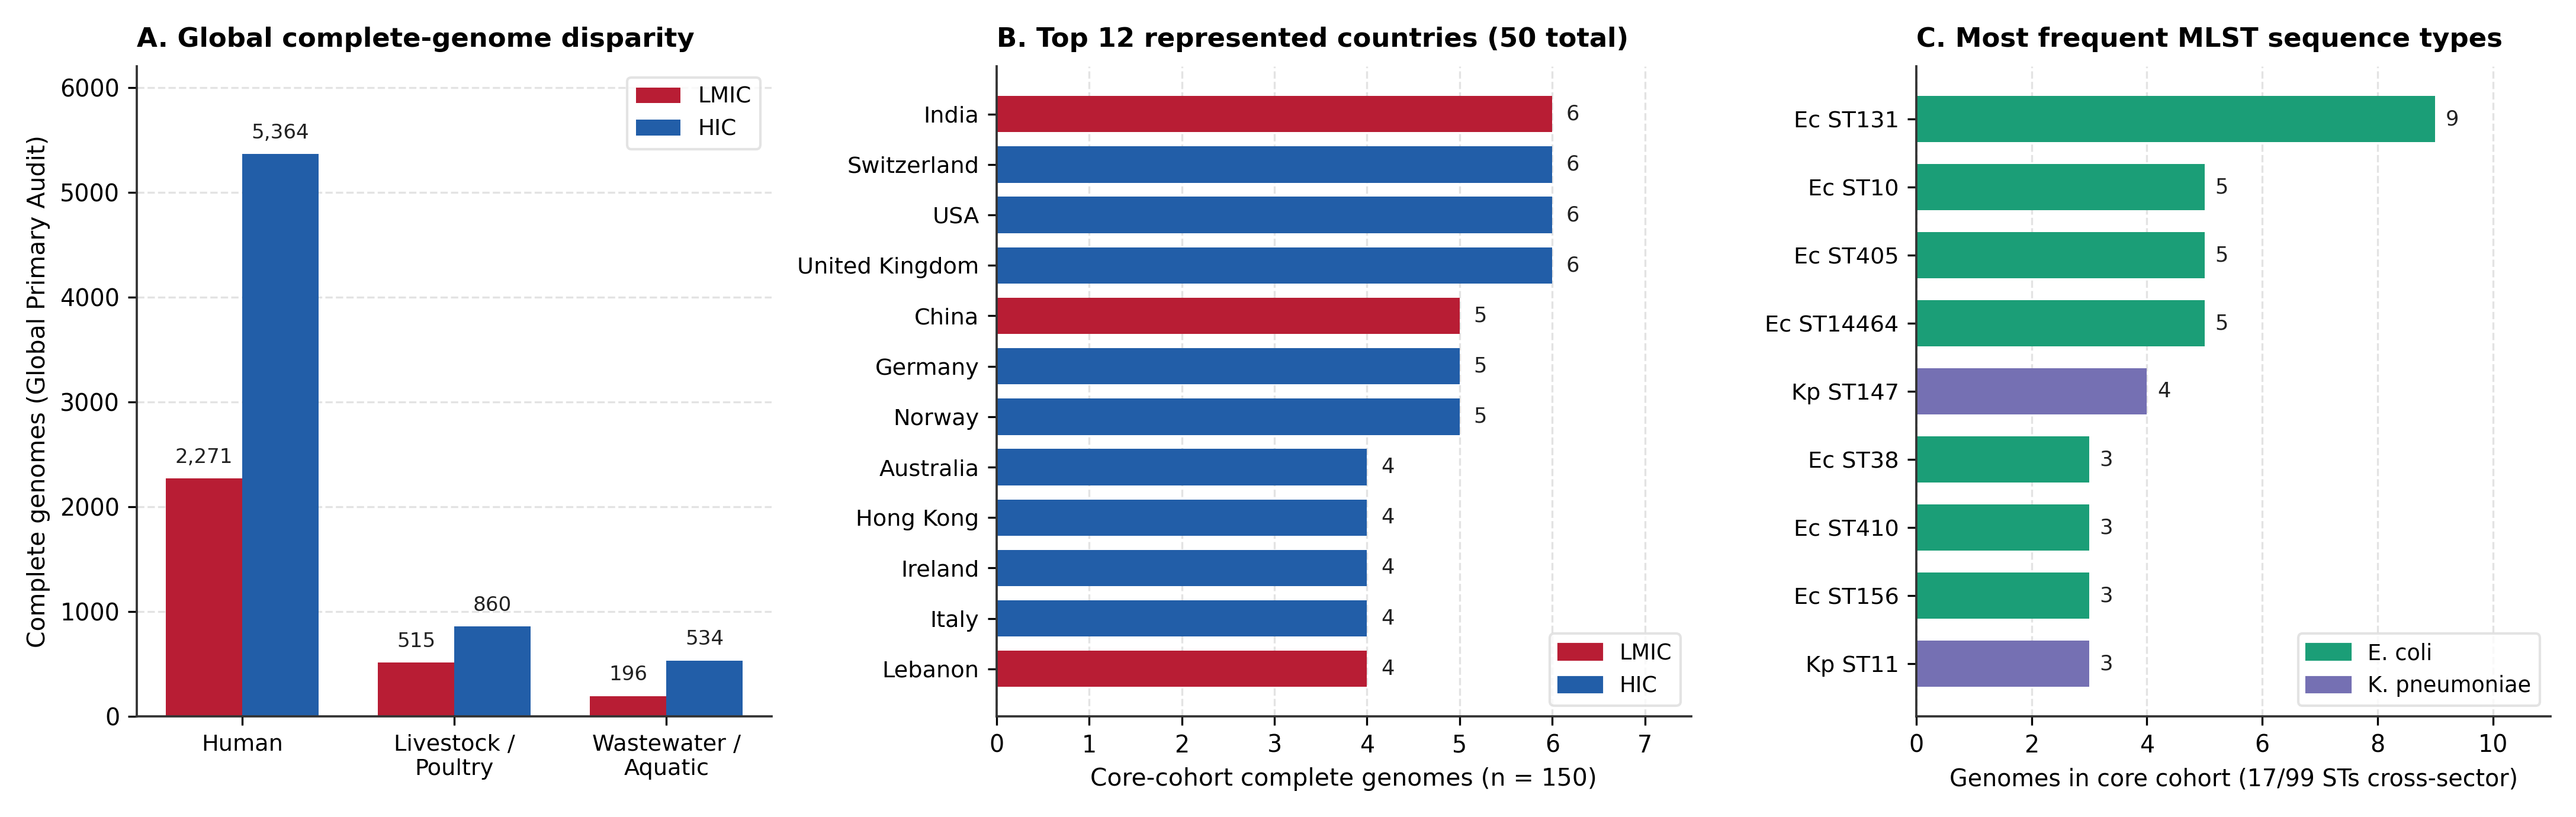
\includegraphics[width=\linewidth]{figures/fig1.png}
  \caption{\textbf{Complete-genome repository counts and stratified sample structure.} (\textbf{A}) Complete genomes in the NCBI Pathogen Detection audit ($n = 10{,}073$; HIC and LMIC classified counts shown). (\textbf{B}) Top 12 represented countries in the BUSCO-passing sample ($n = 150$, 50 countries total). (\textbf{C}) Most frequent MLST sequence types ($\ge 3$ genomes); 17 of 99 distinct STs occurred in $\ge 2$ sectors.}
  \label{fig:cohort}
\end{figure}

\subsection{Population Structure and Clonal Relatedness}

MLST resolved 99 distinct STs (17 in $\ge 2$ sectors; Figure~\ref{fig:cohort}C), including \textit{E.~coli} ST131 ($n = 9$), ST405 ($n = 5$), ST38 ($n = 3$), ST410 ($n = 3$), \textit{K.~pneumoniae} ST147 ($n = 4$), ST11 ($n = 3$), and generalist/cohort-represented types ST10 ($n = 5$), ST14464 ($n = 5$), and ST156 ($n = 3$). ClermonTyping placed 93 \textit{E.~coli} genomes into phylogroups A (26), B1 (19), B2 (19; across Human [12], Wastewater [4], Livestock [3]), D (15), C (5), F (3), clade~I (2), E (2), G (1), and Unknown (1). Among 57 Kleborate-typed \textit{K.~pneumoniae}, 11 scored $\ge 3$ for virulence (7 at score~4: aerobactin plus yersiniabactin without colibactin) across all three sectors.

Across all 9 \textit{E.~coli} ST131 genomes (12,454 unmasked core-SNP sites), 0 of 36 pairs fell within $\le 100$ SNPs; the closest pairs were 117 SNPs (Switzerland vs.\ Germany wastewater), 133 SNPs (South Africa human vs.\ Switzerland wastewater), and 160 SNPs (South Africa human vs.\ Germany wastewater). Within the 1,371 within-chunk SKA2 pairs evaluated (23\% of within-species pairs), \textit{K.~pneumoniae} yielded 1 cross-sector pair across thresholds from 10 to 250 SNPs---the Gothenburg, Sweden ST395 wastewater (\texttt{GCA\_061110345.1}, 2023) and human (\texttt{GCA\_061110765.1}, 2022) pair, confirmed by Snippy at \textbf{2 core SNPs} over 5.58~Mb plus 2 plasmid indels (both Kleborate virulence score~4). Because the 23\% SKA2 subset omitted the ST131 pairs at 117, 133, and 160 SNPs, the SKA2 count of 0 \textit{E.~coli} pairs $\le 250$ SNPs is uninformative for ruling out clonal pairs across the full sample.

\subsection{Strictly Acquired AMR Plasmid Localization}

Within the 150 QC-passing complete or chromosome-level assemblies, \textbf{78.6\% (1,079/1,372)} of strictly acquired AMR hits were plasmid-borne (Figure~\ref{fig:pli}A; Table~\ref{tab:localization}); excluding the two single-contig \texttt{Chromosome}-level records (\texttt{GCA\_026020035.1} and \texttt{GCA\_003963495.1}, which carried 14 chromosomal hits and no assembled plasmid contigs) yielded \textbf{79.5\% (1,079/1,358)}. Because the single BUSCO-excluded genome (\texttt{GCA\_021462125.1}) carried no \texttt{Scope = core} AMR hits, its exclusion did not alter any core-AMR PLI estimate. Complete-genome PLIs for critical genes were supported by multiple independent MOB-suite clusters (Figure~\ref{fig:pli}B): \textit{bla}\textsubscript{NDM-5} (\textbf{1.00}, 10/10, hit-level Wilson 95\% CI 0.72--1.00; 5 clusters, cluster-level Wilson 95\% CI 0.57--1.00), \textit{bla}\textsubscript{KPC-2} (\textbf{1.00}, 8/8, hit-level Wilson CI 0.68--1.00; 5 clusters, cluster-level CI 0.57--1.00), \textit{bla}\textsubscript{OXA-48} (\textbf{0.88}, 7/8, Wilson CI 0.53--0.98; 4 clusters), \textit{bla}\textsubscript{TEM-1} (\textbf{0.86}, 70/81, bootstrap CI 0.78--0.93), \textit{bla}\textsubscript{KPC-3} (\textbf{0.75}, 3/4, Wilson CI 0.30--0.95; 3 clusters), \textit{mcr-1.1} (\textbf{0.73}, 8/11, Wilson CI 0.43--0.90, bootstrap CI 0.50--1.00; 4 clusters), \textit{bla}\textsubscript{CTX-M-55} (\textbf{0.67}, 4/6, Wilson CI 0.30--0.90), \textit{bla}\textsubscript{CTX-M-15} (\textbf{0.60}, 30/50, bootstrap CI 0.47--0.72; 20 clusters), \textit{bla}\textsubscript{NDM-1} (\textbf{0.60}, 3/5, Wilson CI 0.23--0.88), and \textit{bla}\textsubscript{OXA-181} (\textbf{0.20}, 1/5, Wilson CI 0.04--0.62).

Unfiltered modeling on all 4,948 rows (45.8\% plasmid-borne) inflated the \textit{K.~pneumoniae} vs.\ \textit{E.~coli} plasmid OR to 10.26 ($p < 2 \times 10^{-16}$) and created a spurious wastewater OR of 1.50 ($p = 0.0038$). On strictly acquired AMR hits ($n = 1{,}369$ HIC+LMIC), \textit{K.~pneumoniae} retained \textbf{OR 2.58} (95\% CI 1.10--6.04, $p = 0.029$), unchanged under symmetric exclusion (\textbf{OR 2.58}, $p = 0.032$), strengthened after genome $\times$ gene deduplication (\textbf{OR 2.76}, $p = 0.018$), and consistent with gene-stratified Mantel--Haenszel pooling across 41 shared genes (\textbf{MH OR 2.99}, 95\% CI 2.12--4.23; Table~\ref{tab:localization}). Leave-one-country-out checks confirmed no single country drove localization (most influential: India, $\Delta$ plasmid fraction $+0.0083$, $\Delta$ species OR $+0.059$). No difference was detected by sector or income, though wide intervals do not exclude moderate differences.

\begin{table}[!htbp]
\centering
\caption{Plasmid localization of strictly acquired AMR genes across 150 QC-passing complete genomes ($n = 1{,}372$ total hits; $n = 1{,}369$ HIC+LMIC hits in primary logit; $n = 1{,}237$ deduplicated).}
\label{tab:localization}
\footnotesize
\setlength{\tabcolsep}{4.5pt}
\begin{tabularx}{\linewidth}{@{}l X r r r r r@{}}
\toprule
\textbf{Stratum} & \textbf{Category} & \textbf{Plasmid/Tot.} & \textbf{PLI (\%)} & \textbf{Primary OR (95\% CI)} & \textbf{Dedup.\ OR (95\% CI)} & \textbf{MH OR (95\% CI)} \\
\midrule
\textbf{Overall} & Strictly acquired AMR & 1,079 / 1,372 & 78.6 & --- & --- & --- \\
\midrule
\textbf{Species} & \textit{E.~coli}/\textit{Shigella} (ref.) & 574 / 792 & 72.5 & 1.00 & 1.00 & 1.00 \\
 & \textit{K.~pneumoniae} & 505 / 580 & 87.1 & \textbf{2.58 (1.10--6.04)}$^{*}$ & \textbf{2.76 (1.19--6.40)}$^{\dagger}$ & \textbf{2.99 (2.12--4.23)} \\
\midrule
\textbf{Sector} & Human (ref.) & 483 / 604 & 80.0 & 1.00 & 1.00 & 1.00 \\
 & Livestock/Poultry & 249 / 319 & 78.1 & 1.14 (0.48--2.71) & 1.15 (0.48--2.71) & 0.83 (0.56--1.21) \\
 & Wastewater/Aquatic & 347 / 449 & 77.3 & 0.94 (0.36--2.45) & 0.89 (0.36--2.24) & 0.83 (0.60--1.15) \\
\midrule
\textbf{Income} & HIC (ref.) & 583 / 735 & 79.3 & 1.00 & 1.00 & 1.00 \\
 & LMIC & 493 / 634 & 77.8 & 0.93 (0.43--1.97) & 0.99 (0.47--2.06) & 0.90 (0.68--1.20) \\
 & Unclass.\ (Taiwan) & 3 / 3 & 100.0 & Excluded & Excluded & --- \\
\bottomrule
\end{tabularx}
\vspace{2pt}
\raggedright\footnotesize{$^{*}p = 0.029$; $^{\dagger}p = 0.018$. Symmetric exclusion ($n = 1{,}356$ HIC+LMIC; excludes 3 Taiwan hits) gave \textit{Kp} vs.\ \textit{Ec} OR 2.58 (95\% CI 1.09--6.12, $p = 0.032$); all-\texttt{core} sensitivity ($n = 1{,}587$ HIC+LMIC; excludes 11 Taiwan hits) gave OR 0.66 (95\% CI 0.37--1.18, $p = 0.16$).}
\end{table}

\begin{figure}[!htbp]
  \centering
  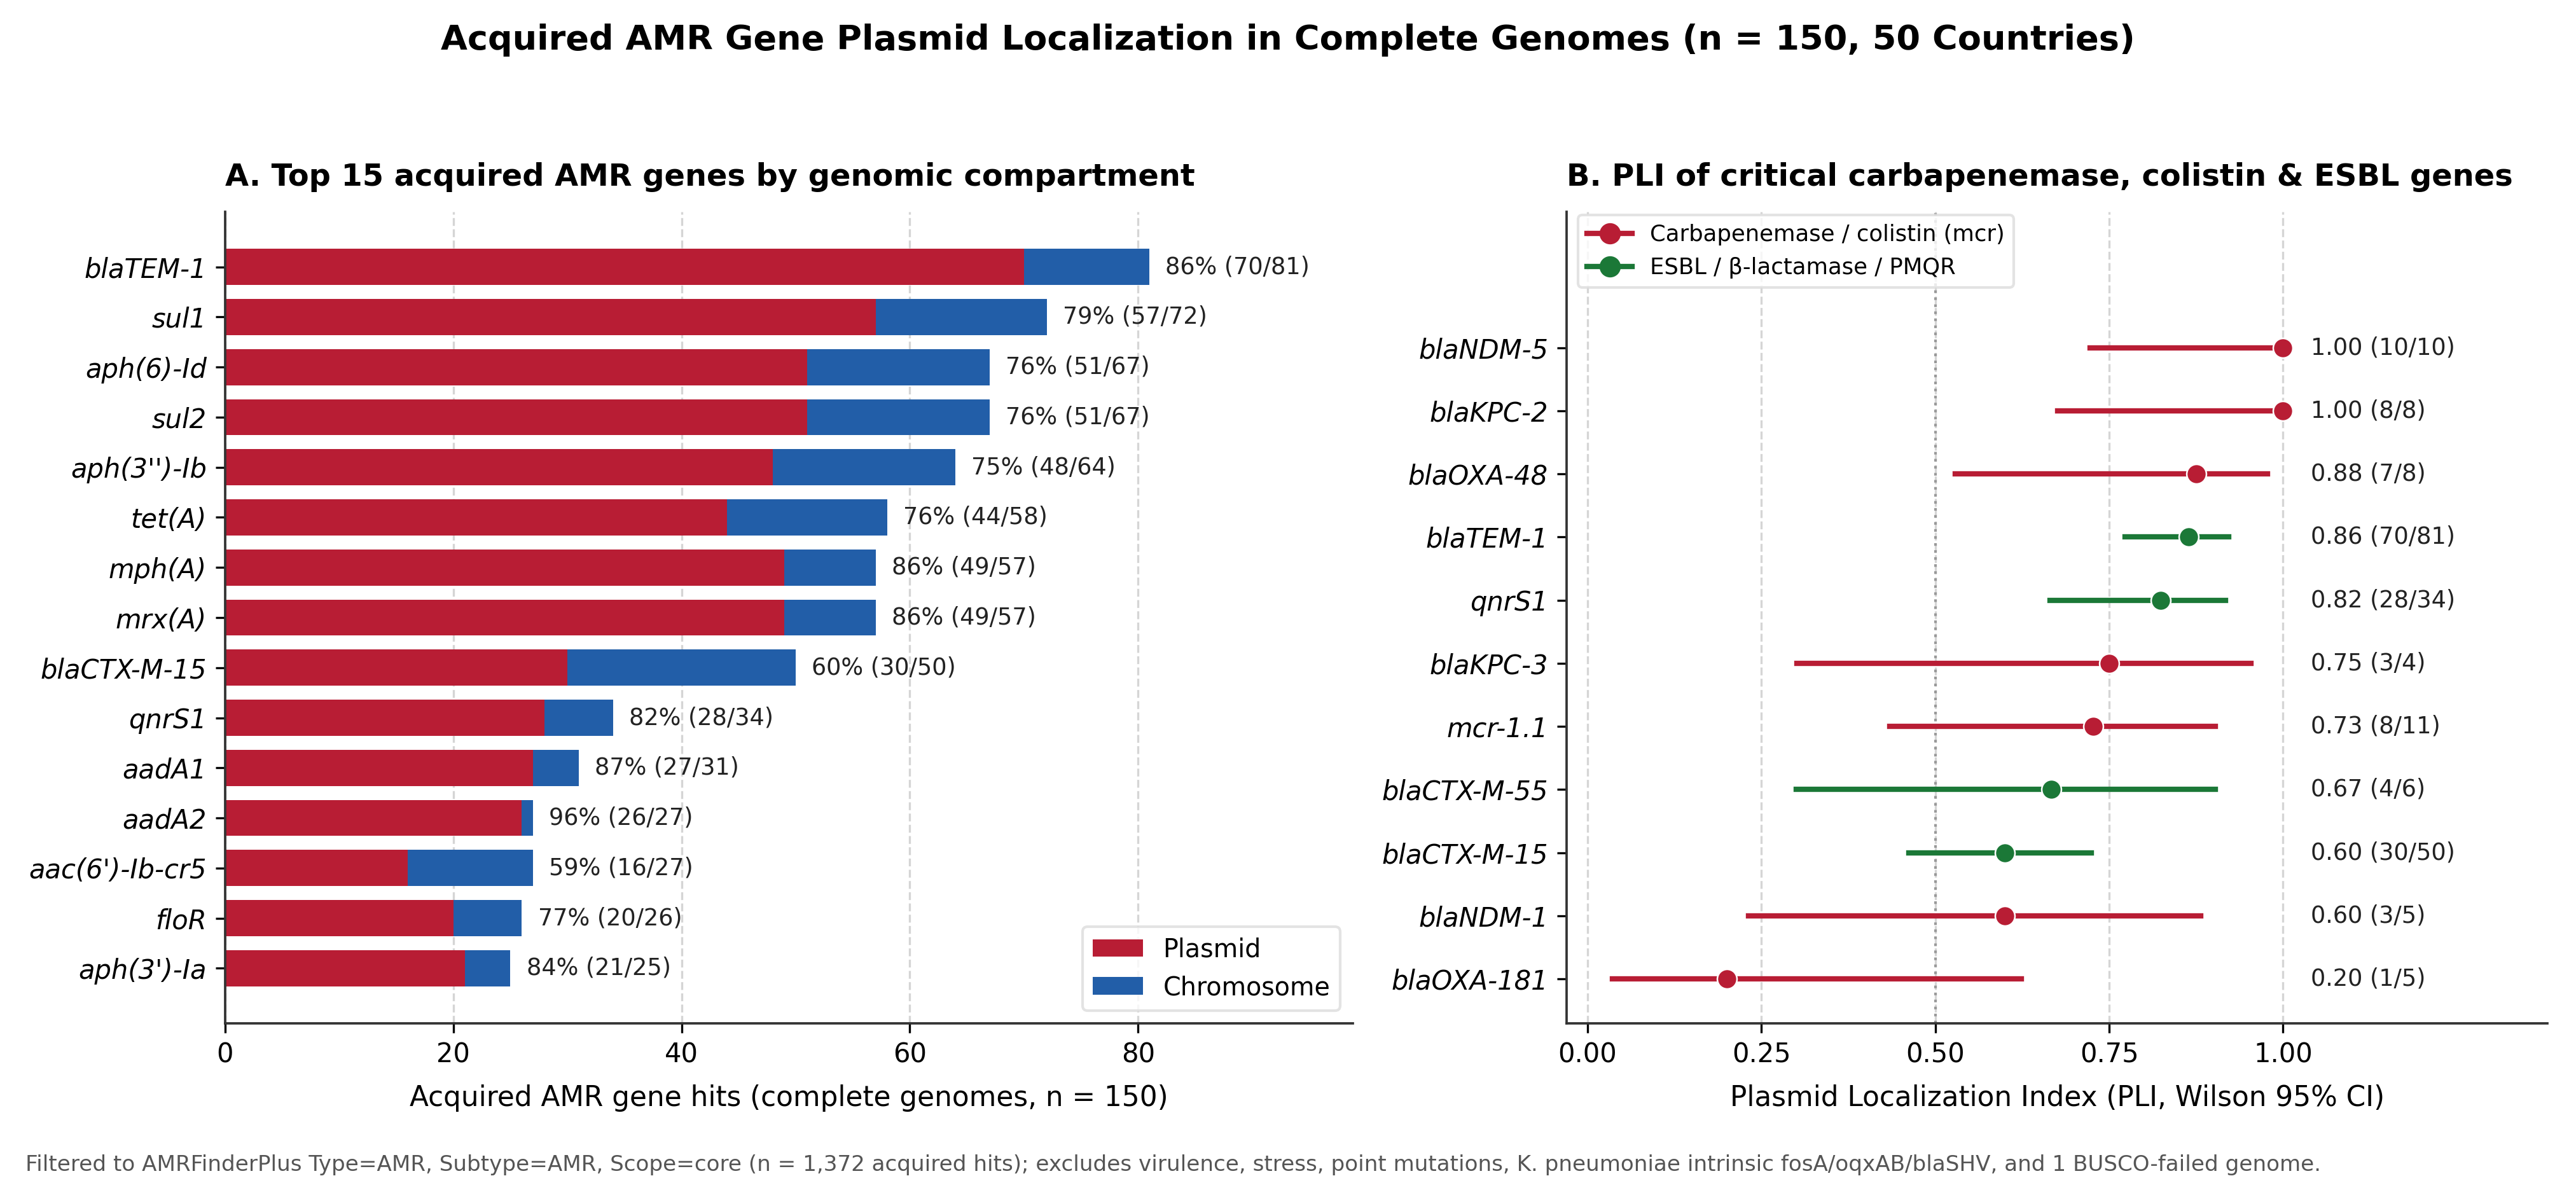
\includegraphics[width=\linewidth]{figures/fig2.png}
  \caption{\textbf{Plasmid localization of strictly acquired AMR genes in complete genomes ($n = 150$).} (\textbf{A}) Top 15 strictly acquired AMR genes by compartment. (\textbf{B}) PLI with hit-level Wilson 95\% CIs for carbapenemase, colistin (\textit{mcr-1.1}), ESBL, and PMQR genes.}
  \label{fig:pli}
\end{figure}

\subsection{Plasmid Cluster Accounting, Permutation Null, and Per-Plasmid Lineages}

Table~\ref{tab:accounting} reconciles all plasmid-cluster and hit denominators. Among non-singleton strictly acquired AMR clusters ($\ge 2$ genomes) in the 150-genome sample, 28 of 34 primary clusters (82.4\%) and 26 of 33 tighter secondary clusters (78.8\%) spanned $\ge 2$ sectors. In 1,000 within-species sector-label permutations, observed counts matched random sector assortment closely (primary: 28 vs.\ 28.87 expected, SD 1.89, $p = 0.757$; secondary: 26 vs.\ 25.25 expected, SD 2.13, $p = 0.452$). Thus, the high multi-sector proportion indicates an \textbf{absence of sector compartmentalization} rather than excess cross-sector sharing above chance. Within individual countries, we observed 5 same-country cross-sector primary plasmid pairs (\texttt{AA002}, \texttt{AA018}, \texttt{AA170}, \texttt{AA402}, \texttt{AA405}; 3 within $\le 2$ years) and 3 same-country secondary pairs (\texttt{AH561}, \texttt{AH818}, \texttt{AI436}; 2 within $\le 2$ years).

In stratified rarefaction (50 replicates per size, $n = 25$--$145$) on the clean 1,372-hit acquired-AMR dataset, plasmid fraction stayed stable across sample sizes (0.778 [SD 0.076] at $n = 25$ to 0.786 [SD 0.005] at $n = 145$), while cross-sector acquired-AMR plasmid clusters rose from 2.94 (SD 1.58) at $n = 25$ to 24.24 (SD 1.58) at $n = 125$ and 27.54 (SD 0.64) at $n = 145$. Per-plasmid cargo inspection (Supplementary Table~S1, 124 individual plasmids; Figure~\ref{fig:network}; Table~\ref{tab:plasmids}) separates multi-lineage unions (e.g., IncI2 \texttt{AA372}: \textit{mcr-1.1} on \texttt{AI350} vs.\ \textit{bla}\textsubscript{KPC-3} on \texttt{AI348}) from single-plasmid co-carriage (e.g., IncFIB/HI1B \texttt{AI436} co-carrying \textit{bla}\textsubscript{NDM-5}+\textit{bla}\textsubscript{CTX-M-15}+\textit{armA} on 332--369~kb molecules across 4 countries). Descriptively, stress resistance genes (\texttt{Type = STRESS}) co-occurred on 39 of 70 (55.7\%) acquired-AMR plasmid clusters.

\begin{table}[!htbp]
\centering
\caption{Reconciliation of hit, plasmid-fraction, and MOB-suite plasmid-cluster denominators across analyses.}
\label{tab:accounting}
\footnotesize
\setlength{\tabcolsep}{4.5pt}
\begin{tabularx}{\linewidth}{@{}X r r r r@{}}
\toprule
\textbf{Dataset / Filter Scope} & \textbf{Genomes} & \textbf{Hits (Plasmid \%)} & \textbf{Total ($\ge 2$ Gen.)} & \textbf{Cross-Sector ($\ge 2$ Sec.)} \\
\midrule
Full MOB-suite output (all plasmids, incl.\ non-AMR) & 151 & NA & 179$^{\dagger}$ & 58 \\
Merged AMRFinderPlus table (unfiltered) & 151 & 4,948 (45.8\%) & 87 (38) & 29 \\
Strictly acquired AMR (primary clusters, $\sim$6\% Mash) & 150 & 1,372 (78.6\%) & 70 (34) & 28 \\
Strictly acquired AMR (secondary clusters, $\sim$2.5\% Mash) & 150 & 1,372 (78.6\%) & 104 (33) & 26 \\
\bottomrule
\end{tabularx}
\vspace{2pt}
\raggedright\footnotesize{$^{\dagger}$The full MOB-suite summary reported total (179) and cross-sector (58) cluster counts without a separate non-singleton denominator; NA = includes plasmids without AMRFinderPlus hits.}
\end{table}

\begin{table}[!htbp]
\centering
\caption{Selected cross-sector and cross-species acquired-AMR plasmid lineages in the 150-genome complete sample (individual plasmid records in Supplementary Table~S1).}
\label{tab:plasmids}
\footnotesize
\setlength{\tabcolsep}{4pt}
\begin{tabularx}{\linewidth}{@{}l l l l r r X@{}}
\toprule
\textbf{Cluster} & \textbf{Replicon(s)} & \textbf{Sectors} & \textbf{Sp.} & \textbf{Pl.\ (Sec.)} & \textbf{Size (kb)} & \textbf{Per-Plasmid Cargo Breakdown} \\
\midrule
\texttt{AA372} & IncI2 & H, L, W & \textit{Ec, Kp} & 4 (2) & 62--75 & \texttt{AI350}: \textit{mcr-1.1} (L/W); \texttt{AI348}: \textit{bla}\textsubscript{KPC-3} (H) \\
\texttt{AA474} & IncI1/B/O/K1 & H, L, W & \textit{Ec} & 9 (8) & 86--138 & 8 sub-lineages; varied \textit{bla}\textsubscript{CTX-M} variants \\
\texttt{AA405} & IncFIB/HI1B/R & H, L, W & \textit{Kp} & 8 (2) & 249--371 & \texttt{AI436}: \textit{bla}\textsubscript{NDM-5}+\textit{CTX-M-15}; \textit{OXA-48}/\textit{NDM-1} \\
\texttt{AA002} & IncL/M & H, L, W & \textit{Kp} & 5 (2) & 64--70 & \texttt{AH539}: \textit{bla}\textsubscript{OXA-48} (63.6~kb, H/W); \texttt{AH529}: \textit{CTX-M-14} (H/L) \\
\texttt{AA277} & IncFIB/FII/R & H, L, W & \textit{Kp} & 6 (1) & 237--338 & \texttt{AI089}: \textit{CTX-M-15}+\textit{OXA-1} (H/W); \textit{NDM-1} (L) \\
\texttt{AA998} & IncHI1A/FIA/X4 & H, L, W & \textit{Ec} & 7 (2) & 186--344 & \texttt{AJ514}/\texttt{516}: \textit{mcr-1.1}/\textit{1.5} (H/L); MDR (W) \\
\texttt{AA338} & IncFIA/FIC & H, W & \textit{Ec, Kp} & 6 (3) & 69--103 & \texttt{AI283}: \textit{bla}\textsubscript{NDM-5}+\textit{rmtB1} (H); \textit{CTX-M-14} (W) \\
\texttt{AA619} & IncX4 & H, L & \textit{Ec, Kp} & 6 (2) & 33--46 & \texttt{AI859}: \textit{mcr-1.1}/\textit{1.26} across 5 countries (H/L) \\
\texttt{AA038} & ColRNAI/X3 & H, W & \textit{Ec, Kp} & 4 (2) & 47--69 & \texttt{AH614}: \textit{bla}\textsubscript{KPC-3} (H); \texttt{AH615}: \textit{SHV-12}+\textit{qnrS1} (W) \\
\texttt{AB595} & Untyped & H, W & \textit{Ec, Kp} & 2 (1) & 6.2--6.2 & \texttt{AK439}: \textit{aph(3'')-Ib}+\textit{aph(6)-Id}+\textit{sul2} (TZ/UG) \\
\bottomrule
\end{tabularx}
\vspace{2pt}
\raggedright\footnotesize{Pl.\ (Sec.) = individual AMR-bearing plasmids (distinct MOB-suite secondary clusters). Sectors: H = Human, L = Livestock/Poultry, W = Wastewater/Aquatic.}
\end{table}

\begin{figure}[!htbp]
  \centering
  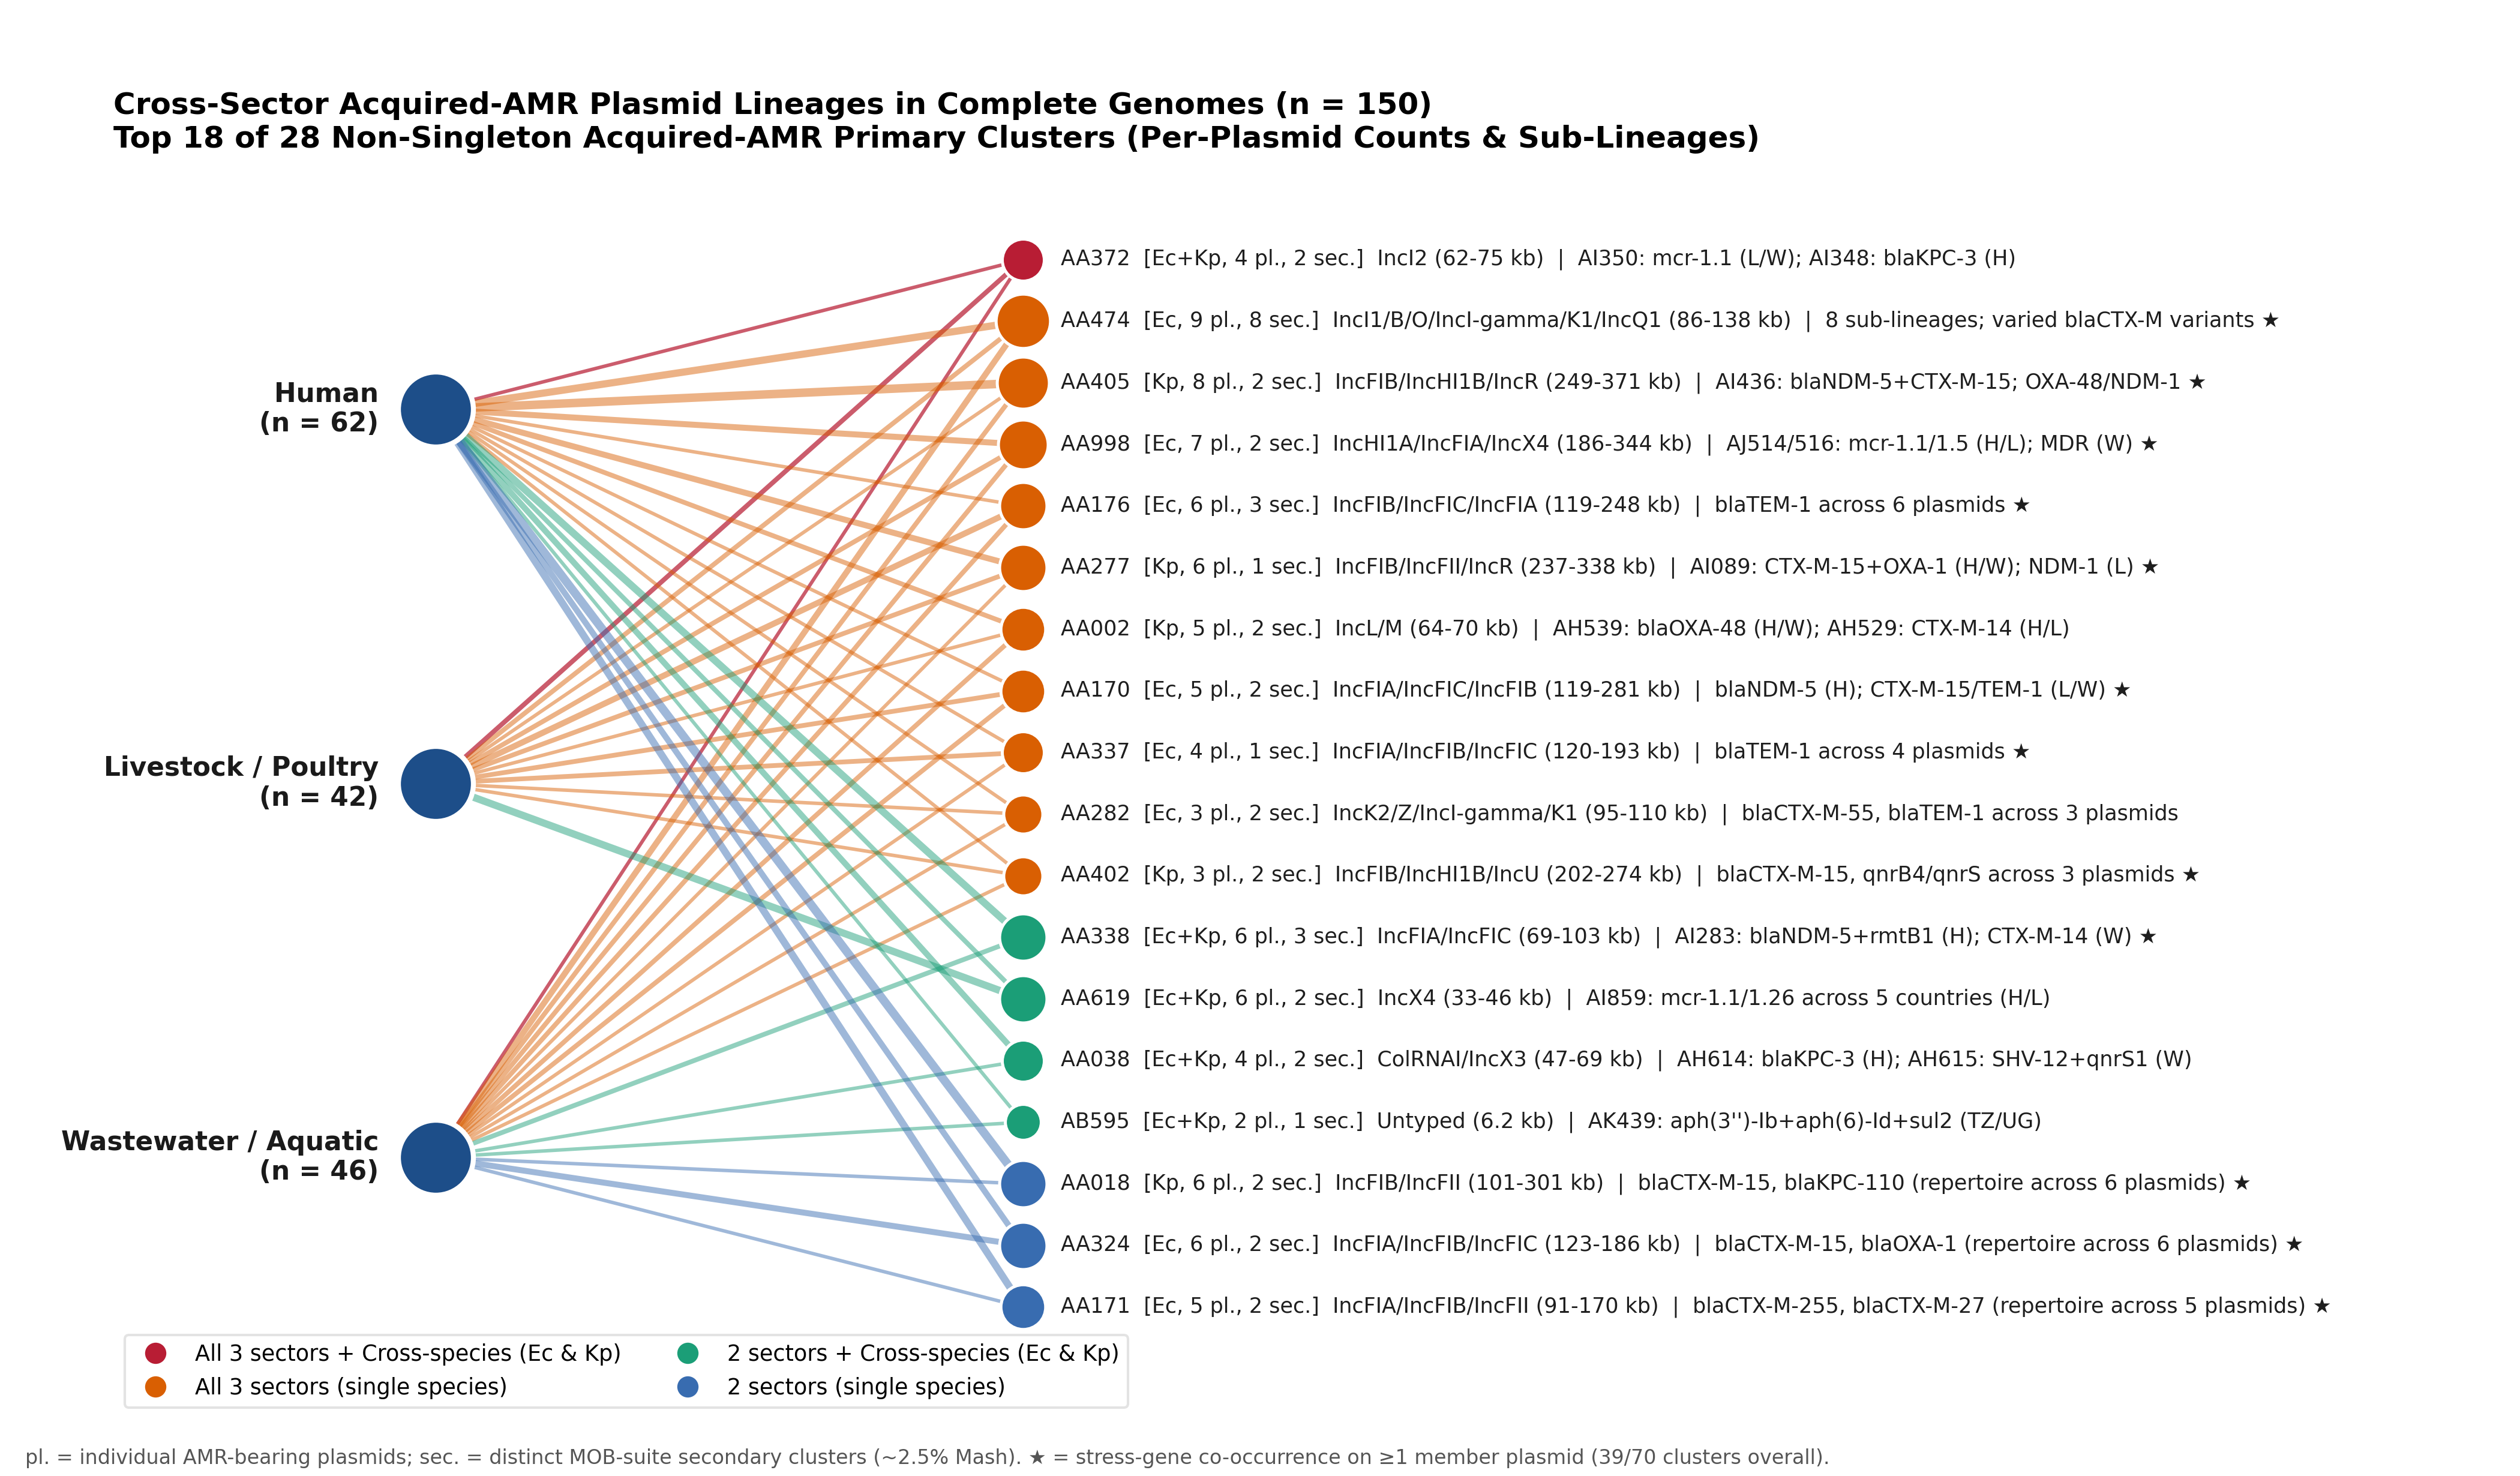
\includegraphics[width=\linewidth]{figures/fig3.png}
  \caption{\textbf{Cross-sector acquired-AMR plasmid lineages in complete genomes ($n = 150$).} Top 18 of 28 non-singleton acquired-AMR primary clusters, annotated with individual plasmid counts, secondary-cluster counts, size ranges, and per-plasmid cargo splits matching Table~\ref{tab:plasmids}. Stars denote stress-gene co-occurrence.}
  \label{fig:network}
\end{figure}

% ==================== 4. DISCUSSION ====================
\section{Discussion}

\takeaway{Key Synthesis}{Across 8,987 complete genomes, Livestock/Poultry reservoirs consistently carry elevated odds of last-resort resistance genes---driven predominantly by \textit{mcr} (OR 1.72--6.72 across specifications)---while in our 150-genome complete sample, strict acquired-AMR filtering reduces the \textit{K.~pneumoniae} vs.\ \textit{E.~coli} plasmid-localization OR fourfold (10.26 to 2.58) and plasmid clusters show no sector compartmentalization in permutation testing.}

Three practical findings emerge from this study. First, the frame-level models separate consistent agricultural signals from country-sensitive income estimates. Livestock/Poultry enrichment of last-resort resistance genes (75.9\% \textit{mcr}) persisted across LMICs alone (OR 2.64), HICs alone (OR 3.63), \textit{mcr} alone (OR 3.43), after removing the UK, China, and USA (OR 6.72), and in the fixed-effects GLM (OR 1.72). By contrast, removing those three countries (63\% of the frame, including China) shifted the LMIC estimate from OR 3.31 to OR 2.63 (95\% CI 0.61--11.34, $p = 0.195$), leaving both reduced statistical power and single-country leverage consistent with the result.

Second, our naive-versus-filtered localization comparison highlights a major methodological pitfall in automated plasmid surveillance. Modeling unfiltered AMRFinderPlus \texttt{--plus} hits inflated the \textit{K.~pneumoniae} vs.\ \textit{E.~coli} plasmid OR from 2.58 to 10.26 and generated a spurious wastewater signal (OR 1.50 vs.\ 0.94). Once strictly filtered---and verified under symmetric intrinsic exclusion (OR 2.58), genome $\times$ gene deduplication (OR 2.76), gene-stratified pooling (MH OR 2.99), and leave-one-country-out checks---localization depended primarily on gene and species, with no detected sector or income difference within our statistical power.

Third, permutation testing and per-plasmid inspection clarify how plasmid connectivity should be interpreted \cite{ludden2019,redondosalvo2020,acman2022}. Because 28/34 primary and 26/33 secondary clusters spanned sectors at rates matching random sector assortment ($p > 0.45$), raw multi-sector cluster percentages indicate an absence of sector compartmentalization rather than excess cross-sector transfer. Per-plasmid tracking of conserved secondary lineages (\texttt{AI436}, \texttt{AH539}, \texttt{AI859}, \texttt{AK439}) separates true multidrug-resistance co-carriage from primary-cluster unions.

% ==================== 5. LIMITATIONS ====================
\section{Limitations}

Structural constraints of the underlying repository and current sample bound interpretation: (1) public NCBI Pathogen Detection repositories reflect uneven national sequencing investments (with the UK, China, and USA contributing 62.8\% of the complete-genome shortlist) and BioProject clustering (such as targeted livestock colistin surveys) rather than probability-sampled surveillance; (2) the regular-expression sector classifier has not yet undergone formal hand-labeled precision/recall validation, and every sector-stratified comparison depends on its accuracy; (3) the unweighted rank-1 sample covers 1.7\% of the 8,987-genome frame (enriching last-resort carriage to $\sim$32\% vs.\ 6.57\%); (4) within-chunk SKA2 covered only 23\% of within-species pairs, ST131 core SNPs were unmasked for recombination, and clonal versus plasmid metrics operate at distinct evolutionary resolutions; and (5) flanking MGE synteny was not assessed. Scaling localization to all 8,987 complete genomes via GenBank replicon headers, validating GenBank versus MOB-suite replicon agreement, running targeted SNP calling across all $\sim$107 same-country cross-sector pairs, adding an ST permutation test, and fitting pooled carbapenemase, single-country leave-one-out, BioProject random-effect, and draft-cohort models are planned prior to peer-reviewed journal submission.

% ==================== 6. DECLARATIONS & SUPPLEMENTARY NOTE ====================
\section{Declarations and Supplementary Note}

\noindent\textbf{Supplementary Note:} An exploratory 50-genome Pakistan pilot (90\% draft WGS; 0/20 complete \textit{K.~pneumoniae}) showed short-contig chromosomal misassignment of \textit{bla}\textsubscript{NDM-1}/\textit{bla}\textsubscript{NDM-7} and identified the \texttt{midstream}/\texttt{stream} and veterinary \texttt{epi\_type='clinical'} metadata rules patched prior to the audit. During QC, CheckM2 failed Python 3.10--3.12 builds (\texttt{scikit-learn==0.23.2}) and CheckM1 failed from OOM/missing indices, leading to substitution with BUSCO v6.1.0 (\texttt{enterobacterales\_odb10}). One divergent Indian wastewater \textit{K.~pneumoniae} genome (\texttt{GCA\_056636575.1}) failed Kleborate with an internal assertion error and remained untyped by MLST. An extended 300-genome manifest (+149 staged rank-2+ assemblies, 0 download failures) is archived for subsequent processing.

\noindent\textbf{Author Contributions:} M.A.K.\ conceived the study, designed the protocol, executed all analyses, and wrote the manuscript. \textbf{Funding \& Competing Interests:} No external grant funding; no competing interests. \textbf{Ethics:} Publicly available de-identified NCBI data; ethical approval not required. \textbf{AI Disclosure:} Large language model assistance was used for code auditing, statistical verification, and manuscript editing; the author verified all outputs and interpretations. \textbf{Data and Code Availability:} Source snapshots were retrieved from \href{https://www.ncbi.nlm.nih.gov/pathogens/docs/isolates_gcp}{NCBI Pathogen Detection} (\texttt{PDG000000004.6463}, \texttt{PDG000000012.2587}, 23 Nov 2026) and the \href{https://api.worldbank.org/v2/country/all?format=json&per_page=300}{World Bank API} (24 Nov 2026). Supplementary Table~S1 (\texttt{TableS1\_per\_plasmid\_cargo\_n150.tsv}), genome accession lists, and analysis scripts are archived at Zenodo (DOI: \href{https://doi.org/10.5281/zenodo.24589690}{10.5281/zenodo.24589690}) and mirrored at \href{https://github.com/ak9287107-star/one-health-amr-connectivity}{github.com/ak9287107-star/one-health-amr-connectivity}.

% ==================== REFERENCES ====================
\bibliographystyle{unsrtnat}
\bibliography{references}

\end{document}
